\documentclass[11pt,a4paper,modern]{FFExercises}
\usepackage[english,greek]{babel}
\usepackage[utf8]{inputenc}
\usepackage{nimbusserif}
\usepackage[T1]{fontenc}
\usepackage{amsmath}
\let\myBbbk\Bbbk
\let\Bbbk\relax
\usepackage[amsbb,subscriptcorrection,zswash,mtpcal,mtphrb,mtpfrak]{mtpro2}
\usepackage{graphicx,multicol,multirow,enumitem,tabularx,mathimatika,gensymb,venndiagram,hhline,longtable,tkz-euclide,fontawesome5,eurosym,tcolorbox,tabularray,tikzpagenodes,relsize,siunitx,eurosym}
\definecolor{xrwma}{HTML}{aa1212}
\usetikzlibrary{calc}
\usetikzlibrary{positioning}
\tcbuselibrary{skins,theorems,breakable}
\renewcommand{\textstigma}{\textsigma\texttau}
\renewcommand{\textdexiakeraia}{}
\usepackage{svg}
\ekthetesdeiktes
\begin{document}

\titlos{Άλγεβρα}{Β' Γυμνασίου}{Εμβαδά βασικών σχημάτων}
\paragraph{Τετράγωνο}
\askhsh Να βρεθεί το εμβαδόν ενός τετραγώνου με πλευρά
\begin{multicols}{2}
\begin{alist}
\item $a=3\si{cm}$
\item $a=4\si{dm}$
\item $a=\sqrt{5}\si{m}$
\item $x=\dfrac{3}{4}\si{mm}$
\item $x=3{,}4\si{km}$
\end{alist}
\end{multicols}
\askhsh Βρείτε την πλευρά του τετραγώνου το οποίο έχει εμβαδόν:
\begin{multicols}{2}
\begin{alist}
\item $E=16\si{cm^2}$
\item $E=49\si{m^2}$
\item $E=10\si{dm^2}$
\item $E=1{,}44\si{km^2}$
\end{alist}
\end{multicols}
\askhsh Ένα τετράγωνο έχει περίμετρο $\Pi=20\si{dm}$.
\begin{alist}
\item Να υπολογίσετε το εμβαδόν του.
\item Μετατρέψτε το εμβαδόν του τετραγώνου σε $\si{cm^2},\si{m^2}$ και $\si{mm^2}$.
\end{alist}
\askhsh Στο παρακάτω σχήμα δίνεται τετράγωνο πλευράς $x\ \si{cm}$ από το οποίο έχουν αποκοπεί 4 ίσα τετράγωνα πλευράς $3\si{cm}$ από κάθε κορυφή του.
\begin{center}
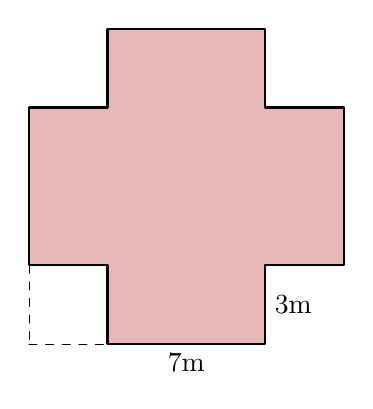
\begin{tikzpicture}
\tkzDefPoints{1/0/A,3/0/B,3/1/C,4/1/D,4/3/E,3/3/F,3/4/G,1/4/H,1/3/I,0/3/J,0/1/K,1/1/L,0/0/O}
\tkzDrawPolygon[line width=0.3mm,fill=xrwma!30](A,B,C,D,E,F,G,H,I,J,K,L)
\tkzDrawSegments[dashed](K,O O,A)
\tkzLabelSegment(A,B){7\si{m}}
\tkzLabelSegment[right](B,C){3\si{m}}
\end{tikzpicture}
\end{center}
\begin{alist}
\item Να βρείτε την πλευρά του αρχικού τετραγώνου.
\item Υπολογίστε το εμβαδόν του χρωματισμένου μέρους.
\end{alist}
\askhsh Το ανάπτυγμα ενός κύβου πλευράς $x\ \si{cm}$ φαίνεται στο παρακάτω σχήμα. Αν η περίμετρος του αναπτύγματος είναι $280\si{cm}$ να βρεθεί:
\begin{center}
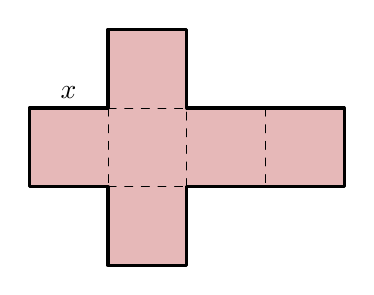
\begin{tikzpicture}
\tkzDefPoints{0/0/A,1/0/B,1/1/C,2/1/D,2/0/E,3/0/F,4/0/G,4/-1/H,3/-1/I,2/-1/J,2/-2/K,1/-2/L,1/-1/M,0/-1/N}
\tkzDrawPolygon[line width=0.4mm,fill=xrwma!30](A,B,C,D,E,F,G,H,I,J,K,L,M,N)
\tkzDrawSegments[dashed](B,M M,J J,E F,I B,E)
\tkzLabelSegment[above](A,B){$x$}
\end{tikzpicture}
\end{center}
\begin{alist}
\item η πλευρά του κύβου.
\item το συνολικό εμβαδόν του κύβου σε $\si{cm^2},\si{dm^2}$ και $\si{mm^2}$.
\end{alist}
\paragraph{Ορθογώνιο}
\askhsh Να βρεθεί το εμβαδόν του ορθογωνίου με διαστάσεις
\begin{alist}
\item $\mu=5\si{m},\ \pi=3\si{m}$
\item $\mu=2{,}5\si{dm},\ \pi=8\si{dm}$
\item $\mu=\sqrt{2}\si{cm},\ \pi=\sqrt{8}\si{cm}$
\item $\mu=10\si{cm},\ \pi=0{,}7\si{dm}$
\item $\mu=5{,}4\si{dm},\ \pi=45\si{cm}$
\item $\mu=\dfrac{2}{5}\si{m},\ \pi=\dfrac{12}{5}\si{m}$
\end{alist}
\askhsh Για τα παρακάτω ορθογώνια δίνεται το εμβαδόν και μία από τις δύο διαστάσεις. Υπολογίστε την πλευρά που λείπει.
\begin{alist}
\item $E=12\si{m^2},\ \mu=4\si{m}$
\item $E=40\si{cm^2},\ \pi=8\si{cm}$
\item $E=14\si{dm^2},\ \mu=5\si{dm}$
\item $E=54\si{m^2},\ \pi=90\si{dm}$
\item $E=\sqrt{48}\si{mm^2},\mu=\sqrt{3}\si{mm^2}$
\item $E=50\si{cm^2},\ \pi=200\si{mm}$
\item $E=4\text{ στρέμματα},\ \pi=50\si{m}$
\end{alist}
\askhsh Συμπληρώστε τον παρακάτω πίνακα.
\begin{center}
\begin{mytblr}{}
Εμβαδόν & Μήκος & Πλάτος\\
  & $4\si{dm}$ & $5\si{dm}$\\
$24\si{m^2}$ &  & $8\si{m}$\\
$100\si{cm^2}$ & $25\si{cm}$ & \\
$3$ στρέμματα & $90\si{m}$ &  \\
  & $45\si{cm}$ & $25\si{cm}$ \\
$144\si{dm^2}$ & $240\si{cm}$ &  \\
\end{mytblr}
\end{center}
\askhsh Ένα ορθογώνιο έχει περίμετρο $30\si{m}$ και πλάτος $8\si{m}$. Να βρεθεί το εμβαδόν του.\\\\
\askhsh Ένα ορθογώνιο έχει διαστάσεις $\mu=32\si{cm}$ και $\pi=18\si{cm}$ και ίση περίμετρο με ένα τετράγωνο. Να βρεθεί:
\begin{alist}
\item το εμβαδόν του ορθογωνίου.
\item το εμβαδόν του τετραγώνου.
\end{alist}
\paragraph{Παραλληλόγραμμο}
\askhsh Δίνεται παραλληλόγραμμο $AB\varGamma\varDelta$ με $AB=8\si{cm}, A\varDelta=6\si{cm}$ και $AK=4\si{cm}$ όπως φαίνεται στο παρακάτω σχήμα. Να βρείτε:
\begin{center}
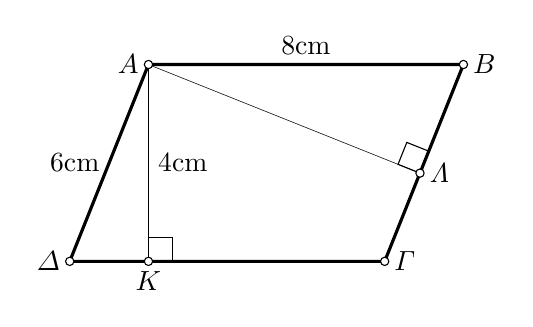
\begin{tikzpicture}
\tkzDefPoints{1/2.5/A,5/2.5/B,4/0/C,0/0/D,1/0/K}
\tkzDrawPolygon[line width=0.4mm](A,B,C,D)
\tkzDefPointBy[projection=onto B--C](A)\tkzGetPoint{L}
\tkzDrawSegments(A,K A,L)
\tkzLabelPoint[left](A){$A$}
\tkzLabelPoint[right](B){$B$}
\tkzLabelPoint[right](C){$\varGamma$}
\tkzLabelPoint[left](D){$\varDelta$}
\tkzLabelPoint[below](K){$K$}
\tkzLabelPoint[right](L){$\varLambda$}
\tkzMarkRightAngle[size=0.3](C,K,A)
\tkzMarkRightAngle[size=0.3](B,L,A)
\tkzLabelSegment[above](A,B){$8\si{cm}$}
\tkzLabelSegment[right](A,K){$4\si{cm}$}
\tkzLabelSegment[left](A,D){$6\si{cm}$}
\tkzDrawPoints[size=3,fill=white](A,B,C,D,K,L)
\end{tikzpicture}
\end{center}
\begin{alist}
\item το εμβαδόν του παραλληλογράμμου.
\item το ύψος $A\varLambda$.
\end{alist}

\askhsh Το παραλληλόγραμμο $AB\varGamma\varDelta$ του παρακάτω σχήματος έχει $\varGamma\varDelta=20\si{dm}, A\varLambda=15\si{dm}$ και $AK=12\si{dm}$. Να βρείτε:
\begin{center}
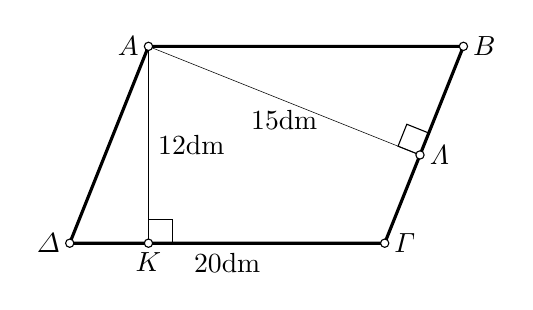
\begin{tikzpicture}
\tkzDefPoints{1/2.5/A,5/2.5/B,4/0/C,0/0/D,1/0/K}
\tkzDrawPolygon[line width=0.4mm](A,B,C,D)
\tkzDefPointBy[projection=onto B--C](A)\tkzGetPoint{L}
\tkzDrawSegments(A,K A,L)
\tkzLabelPoint[left](A){$A$}
\tkzLabelPoint[right](B){$B$}
\tkzLabelPoint[right](C){$\varGamma$}
\tkzLabelPoint[left](D){$\varDelta$}
\tkzLabelPoint[below](K){$K$}
\tkzLabelPoint[right](L){$\varLambda$}
\tkzMarkRightAngle[size=0.3](C,K,A)
\tkzMarkRightAngle[size=0.3](B,L,A)
\tkzLabelSegment[below](C,D){$20\si{dm}$}
\tkzLabelSegment[right](A,K){$12\si{dm}$}
\tkzLabelSegment[below](A,L){$15\si{dm}$}
\tkzDrawPoints[size=3,fill=white](A,B,C,D,K,L)
\end{tikzpicture}
\end{center}
\begin{alist}
\item το εμβαδόν του παραλληλογράμμου σε $\si{dm^2}$ και $\si{m^2}$.
\item την περίμετρο του παραλληλογράμμου.
\end{alist}
\paragraph{Τρίγωνο - Ορθογώνιο τρίγωνο}
\askhsh Δίνεται τρίγωνο $AB\varGamma$ με πλευρές $AB=10\si{cm},B\varGamma=15\si{cm}$ και ύψος $A\varDelta=9\si{cm}$.
\begin{center}
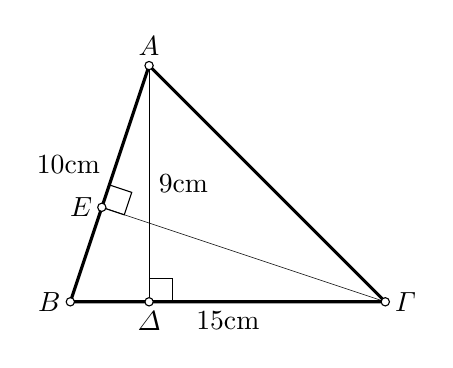
\begin{tikzpicture}
\tkzDefPoints{0/0/B,4/0/C,1/3/A,1/0/D}
\tkzDrawPolygon[line width=0.4mm](A,B,C)
\tkzDefPointBy[projection=onto A--B](C)
\tkzGetPoint{E}
\tkzDrawSegments(A,D C,E)
\tkzMarkRightAngle[size=.3](C,D,A)
\tkzMarkRightAngle[size=.3](C,E,A)
\tkzDrawPoints[size=3,fill=white](A,B,C,D,E)
\tkzLabelPoint[above](A){$A$}
\tkzLabelPoint[left](B){$B$}
\tkzLabelPoint[right](C){$\varGamma$}
\tkzLabelPoint[below](D){$\varDelta$}
\tkzLabelPoint[left](E){$E$}
\tkzLabelSegment[below](B,C){$15\si{cm}$}
\tkzLabelSegment[above left](A,B){$10\si{cm}$}
\tkzLabelSegment[right](A,D){$9\si{cm}$}
\end{tikzpicture}
\end{center}
Να υπολογίσετε:
\begin{alist}
\item το εμβαδόν του τριγώνου σε $\si{cm^2},\si{dm^2}$ και $\si{mm^2}$.
\item το ύψος $\varGamma E$.
\end{alist}
\paragraph{Τραπέζιο}
\askhsh Συμπληρώστε τον παρακάτω πίνακα.
\begin{center}
\begin{mytblr}{row{1}={m}}
Εμβαδόν & {μικρή\\βάση $\beta$} & {Μεγάλη\\βάση $B$} & ύψος $\upsilon$\\
  & $4\si{dm}$ & $8\si{dm}$ & $3\si{dm}$ \\
$48\si{cm^2}$ &  & $10\si{cm}$ & $4\si{cm}$\\
$120\si{m^2}$ & $40\si{m}$ &  & $8\si{m}$ \\
$35\si{mm^2}$ & $7\si{m}$ & $20\si{mm}$ & \\
  & $7\si{dm}$ & $50\si{cm}$ & $200\si{mm}$ \\
$80\si{m^2}$ &  & $1200\si{cm}$ & $160\si{dm}$\\
$45\si{cm^2}$ & $0{,}9\si{m}$ &  & $1\si{dm}$ \\
$240\si{mm^2}$ & $0{,}8\si{dm}$ & $2\si{cm}$ & \\
\end{mytblr}
\end{center}
\paragraph{Προβλήματα}
\askhsh Στο παρακάτω σχήμα βλέπουμε το αρχιτεκτονικό σχέδιο της κάτοψης ενός σπιτιού, με τις διαστάσεις των διάφορων δωματίων. Να υπολογίσετε:
\begin{center}
\includesvg[width=\linewidth]{spiti_import}
\end{center}
\begin{alist}
\item το εμβαδόν του κάθε χώρου μέσα στο σπίτι.
\item το εμβαδόν του μπαλκονιού.
\item τη συνολική αξία αγοράς του σπιτιού, αν γνωρίζουμε ότι πωλείται με $450$\euro/$\si{m^2}$.
\end{alist}
\paragraph{Συνδυαστικά θέματα}
\askhsh Η περίμετρος του παρακάτω σχήματος είναι $51\si{cm}$. Να υπολογίσετε το εμβαδόν του.
\begin{center}
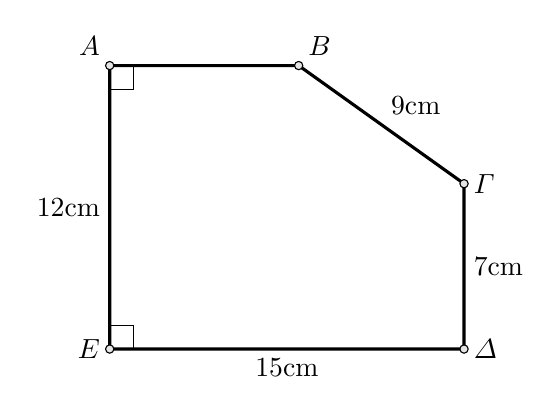
\begin{tikzpicture}
\tkzDefPoints{0/0/E,4.5/0/D,4.5/2.1/C,2.4/3.6/B,0/3.6/A}
\tkzDrawPolygon[line width=0.4mm](A,B,C,D,E)
\tkzMarkRightAngle[size=.3](E,A,B)
\tkzMarkRightAngle[size=.3](D,E,A)
\tkzLabelSegment[left](A,E){$12\si{cm}$}
\tkzLabelSegment[below](D,E){$15\si{cm}$}
\tkzLabelSegment[right](D,C){$7\si{cm}$}
\tkzLabelSegment[above right](B,C){$9\si{cm}$}
\tkzDrawPoints[size=3](A,B,C,D,E)
\tkzLabelPoint[above left](A){$A$}
\tkzLabelPoint[above right](B){$B$}
\tkzLabelPoint[right](C){$\varGamma$}
\tkzLabelPoint[right](D){$\varDelta$}
\tkzLabelPoint[left](E){$E$}
\end{tikzpicture}
\end{center}
\end{document}
